\documentclass{standalone}
\usepackage{tikz}
\usetikzlibrary{patterns, positioning}

\begin{document}
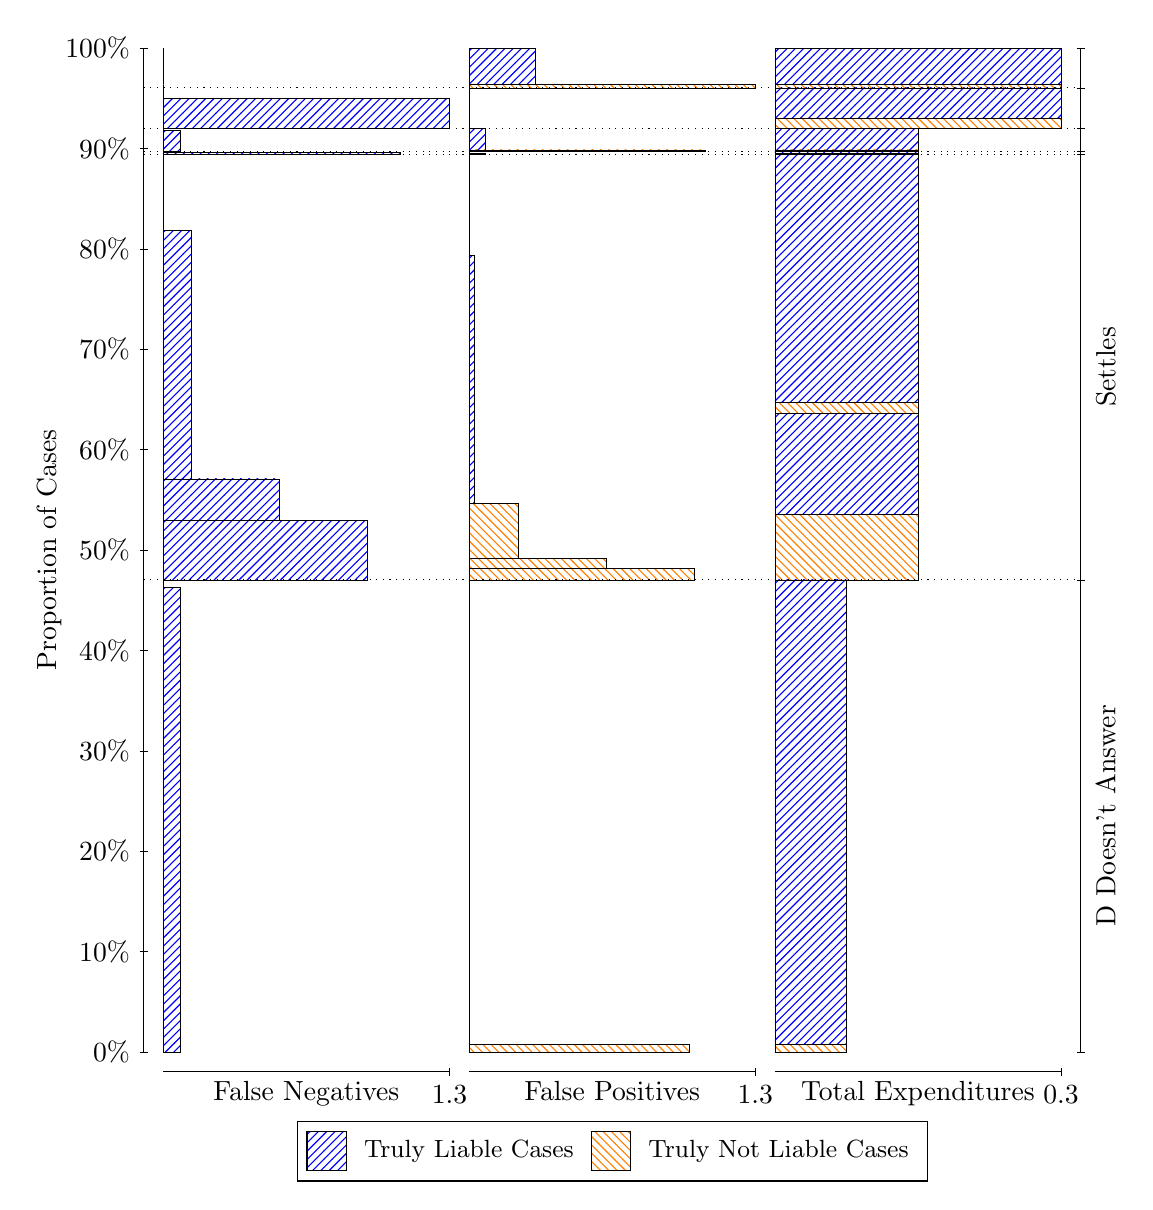
\begin{tikzpicture}
\draw[black, very thin] (1.5,1.75) -- (1.5,14.5);
\node[rotate=90, anchor=center] at (0.3, 8.125) {Proportion of Cases};
\draw[black, very thin] (1.45,1.75) -- (1.55,1.75);
\node[anchor=east] at (1.45, 1.75) {0\%};
\draw[black, very thin] (1.45,3.025) -- (1.55,3.025);
\node[anchor=east] at (1.45, 3.025) {10\%};
\draw[black, very thin] (1.45,4.3) -- (1.55,4.3);
\node[anchor=east] at (1.45, 4.3) {20\%};
\draw[black, very thin] (1.45,5.575) -- (1.55,5.575);
\node[anchor=east] at (1.45, 5.575) {30\%};
\draw[black, very thin] (1.45,6.85) -- (1.55,6.85);
\node[anchor=east] at (1.45, 6.85) {40\%};
\draw[black, very thin] (1.45,8.125) -- (1.55,8.125);
\node[anchor=east] at (1.45, 8.125) {50\%};
\draw[black, very thin] (1.45,9.4) -- (1.55,9.4);
\node[anchor=east] at (1.45, 9.4) {60\%};
\draw[black, very thin] (1.45,10.675) -- (1.55,10.675);
\node[anchor=east] at (1.45, 10.675) {70\%};
\draw[black, very thin] (1.45,11.95) -- (1.55,11.95);
\node[anchor=east] at (1.45, 11.95) {80\%};
\draw[black, very thin] (1.45,13.225) -- (1.55,13.225);
\node[anchor=east] at (1.45, 13.225) {90\%};
\draw[black, very thin] (1.45,14.5) -- (1.55,14.5);
\node[anchor=east] at (1.45, 14.5) {100\%};

\draw[black, very thin] (13.4,1.75) -- (13.4,14.5);
\draw[black, very thin] (13.35,1.75) -- (13.45,1.75);
\node[anchor=west] at (13.35, 1.75) {};
\draw[black, very thin] (13.35,7.7461) -- (13.45,7.7461);
\node[anchor=west] at (13.35, 7.7461) {};
\draw[black, very thin] (13.35,13.153) -- (13.45,13.153);
\node[anchor=west] at (13.35, 13.153) {};
\draw[black, very thin] (13.35,13.185) -- (13.45,13.185);
\node[anchor=west] at (13.35, 13.185) {};
\draw[black, very thin] (13.35,13.477) -- (13.45,13.477);
\node[anchor=west] at (13.35, 13.477) {};
\draw[black, very thin] (13.35,13.994) -- (13.45,13.994);
\node[anchor=west] at (13.35, 13.994) {};
\draw[black, very thin] (13.35,14.5) -- (13.45,14.5);
\node[anchor=west] at (13.35, 14.5) {};

\draw[black, very thin, pattern color=blue, pattern=north east lines] (1.75,1.75) rectangle (1.9596,7.6492);
\draw[black, very thin, pattern color=orange, pattern=north west lines] (1.75,7.6492) rectangle (1.75,7.7461);
\draw[black, very thin, pattern color=blue, pattern=north east lines] (1.75,7.7461) rectangle (4.3353,8.5051);
\draw[black, very thin, pattern color=blue, pattern=north east lines] (1.75,8.5051) rectangle (3.2173,9.0295);
\draw[black, very thin, pattern color=blue, pattern=north east lines] (1.75,9.0295) rectangle (2.0994,12.185);
\draw[black, very thin, pattern color=orange, pattern=north west lines] (1.75,12.185) rectangle (1.75,13.153);
\draw[black, very thin, pattern color=blue, pattern=north east lines] (1.75,13.153) rectangle (4.7545,13.176);
\draw[black, very thin, pattern color=orange, pattern=north west lines] (1.75,13.176) rectangle (1.75,13.185);
\draw[black, very thin, pattern color=blue, pattern=north east lines] (1.75,13.185) rectangle (1.9596,13.455);
\draw[black, very thin, pattern color=orange, pattern=north west lines] (1.75,13.455) rectangle (1.75,13.477);
\draw[black, very thin, pattern color=blue, pattern=north east lines] (1.75,13.477) rectangle (5.3833,13.857);
\draw[black, very thin, pattern color=orange, pattern=north west lines] (1.75,13.857) rectangle (1.75,13.994);
\draw[black, very thin, pattern color=orange, pattern=north west lines] (1.75,13.994) rectangle (1.75,14.037);
\draw[black, very thin, pattern color=blue, pattern=north east lines] (1.75,14.037) rectangle (1.75,14.5);
\draw[black, very thin, pattern color=orange, pattern=north west lines] (5.6333,1.75) rectangle (8.4282,1.8469);
\draw[black, very thin, pattern color=blue, pattern=north east lines] (5.6333,1.8469) rectangle (5.6333,7.7461);
\draw[black, very thin, pattern color=orange, pattern=north west lines] (5.6333,7.7461) rectangle (8.4981,7.8878);
\draw[black, very thin, pattern color=orange, pattern=north west lines] (5.6333,7.8878) rectangle (7.3801,8.0226);
\draw[black, very thin, pattern color=orange, pattern=north west lines] (5.6333,8.0226) rectangle (6.2622,8.7145);
\draw[black, very thin, pattern color=blue, pattern=north east lines] (5.6333,8.7145) rectangle (5.7032,11.87);
\draw[black, very thin, pattern color=blue, pattern=north east lines] (5.6333,11.87) rectangle (5.6333,13.153);
\draw[black, very thin, pattern color=orange, pattern=north west lines] (5.6333,13.153) rectangle (5.8429,13.162);
\draw[black, very thin, pattern color=blue, pattern=north east lines] (5.6333,13.162) rectangle (5.6333,13.185);
\draw[black, very thin, pattern color=orange, pattern=north west lines] (5.6333,13.185) rectangle (8.6378,13.207);
\draw[black, very thin, pattern color=blue, pattern=north east lines] (5.6333,13.207) rectangle (5.8429,13.477);
\draw[black, very thin, pattern color=orange, pattern=north west lines] (5.6333,13.477) rectangle (5.6333,13.614);
\draw[black, very thin, pattern color=blue, pattern=north east lines] (5.6333,13.614) rectangle (5.6333,13.994);
\draw[black, very thin, pattern color=orange, pattern=north west lines] (5.6333,13.994) rectangle (9.2667,14.037);
\draw[black, very thin, pattern color=blue, pattern=north east lines] (5.6333,14.037) rectangle (6.4718,14.5);
\draw[black, very thin, pattern color=orange, pattern=north west lines] (9.5167,1.75) rectangle (10.425,1.8469);
\draw[black, very thin, pattern color=blue, pattern=north east lines] (9.5167,1.8469) rectangle (10.425,7.7461);
\draw[black, very thin, pattern color=orange, pattern=north west lines] (9.5167,7.7461) rectangle (11.333,8.5728);
\draw[black, very thin, pattern color=blue, pattern=north east lines] (9.5167,8.5728) rectangle (11.333,9.8563);
\draw[black, very thin, pattern color=orange, pattern=north west lines] (9.5167,9.8563) rectangle (11.333,9.9979);
\draw[black, very thin, pattern color=blue, pattern=north east lines] (9.5167,9.9979) rectangle (11.333,13.153);
\draw[black, very thin, pattern color=orange, pattern=north west lines] (9.5167,13.153) rectangle (11.333,13.162);
\draw[black, very thin, pattern color=blue, pattern=north east lines] (9.5167,13.162) rectangle (11.333,13.185);
\draw[black, very thin, pattern color=orange, pattern=north west lines] (9.5167,13.185) rectangle (11.333,13.207);
\draw[black, very thin, pattern color=blue, pattern=north east lines] (9.5167,13.207) rectangle (11.333,13.477);
\draw[black, very thin, pattern color=orange, pattern=north west lines] (9.5167,13.477) rectangle (13.15,13.614);
\draw[black, very thin, pattern color=blue, pattern=north east lines] (9.5167,13.614) rectangle (13.15,13.994);
\draw[black, very thin, pattern color=orange, pattern=north west lines] (9.5167,13.994) rectangle (13.15,14.037);
\draw[black, very thin, pattern color=blue, pattern=north east lines] (9.5167,14.037) rectangle (13.15,14.5);
\draw[black, dotted] (1.5,7.7461) -- (13.4,7.7461);
\draw[black, dotted] (1.5,13.153) -- (13.4,13.153);
\draw[black, dotted] (1.5,13.185) -- (13.4,13.185);
\draw[black, dotted] (1.5,13.477) -- (13.4,13.477);
\draw[black, dotted] (1.5,13.994) -- (13.4,13.994);
\draw[black, very thin] (1.75,1.5) -- (5.3833,1.5);
\node[anchor=north] at (3.5667, 1.5) {False Negatives};
\draw[black, very thin] (5.3833,1.45) -- (5.3833,1.55);
\node[anchor=north] at (5.3833, 1.45) {1.3};

\draw[black, very thin] (5.6333,1.5) -- (9.2667,1.5);
\node[anchor=north] at (7.45, 1.5) {False Positives};
\draw[black, very thin] (9.2667,1.45) -- (9.2667,1.55);
\node[anchor=north] at (9.2667, 1.45) {1.3};

\draw[black, very thin] (9.5167,1.5) -- (13.15,1.5);
\node[anchor=north] at (11.333, 1.5) {Total Expenditures};
\draw[black, very thin] (13.15,1.45) -- (13.15,1.55);
\node[anchor=north] at (13.15, 1.45) {0.3};

\node[black, centered, rotate=90] at (13.72, 4.748) {D Doesn't Answer};
\node[black, centered, rotate=90] at (13.72, 10.45) {Settles};





\draw (7.449999999999999,1.5) node[draw=none] (baseCoordinate) {};
\begin{scope}[align=center]
        \matrix[scale=0.5, draw=black, below=0.5cm of baseCoordinate, nodes={draw}, column sep=0.1cm]{
            \node[rectangle, draw, minimum width=0.5cm, minimum height=0.5cm, pattern=north east lines, pattern color=blue] {}; &
            \node[draw=none, font=\small] (B) {Truly Liable Cases}; &
            \node[rectangle, draw, minimum width=0.5cm, minimum height=0.5cm, pattern=north west lines, pattern color=orange] {}; &
            \node[draw=none, font=\small] (B) {Truly Not Liable Cases}; \\
            };
\end{scope}

\end{tikzpicture}
\end{document}